\section{Marco Teórico} %O marco Teórico, que se yo
El Procesamiento de Lenguaje Natural (NPL por sus siglas en inglés) es un campo de las Ciencias de Computación y la Lingüística que trata con métodos para analizar, modelar y entender el lenguaje humano.\\
\begin{figure}[H]
\begin{centering}
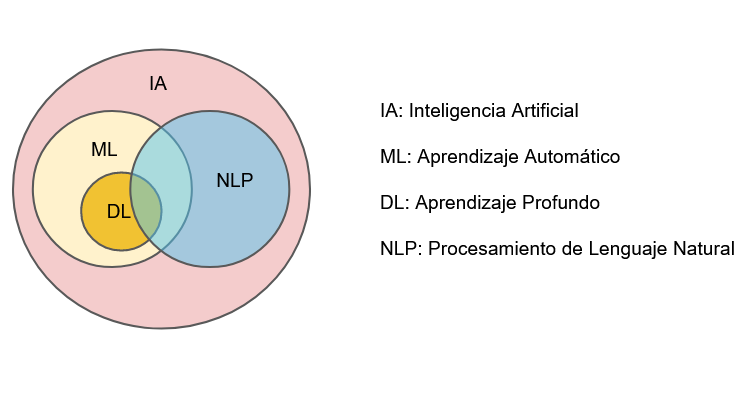
\includegraphics[angle=0,width=0.3\textwidth]{Figuras/NLP.png}
\par \end{centering}
\caption[Procesamiento de Lenguaje Natural]{Procesamiento de Lenguaje Natural. \textbf{Fuente:} Propia}
\label{NLP}
\end{figure}

Existen varios métodos utilizados a lo largo de la historia del Procesamiento de Lenguaje Natural.\\
Los primeros intentos fueron mediante reglas de acciones manuales por medio de árboles de decisión, conocidos como métodos heurísticos o basados en reglas. Este método requiere que los desarrolladores tengan experiencia en el dominio del problema para formular las reglas que puedan ser incorporadas al programa, utilizan bastante los diccionarios y las expresiones regulares.\\
\indent Posteriormente vinieron los métodos basados en aprendizaje automático, como la clasificación y regresión, que son utilizados con frecuencia en NLP.\\
\indent Finalmente, el Aprendizaje profundo o Deep learning(DL), una evolución más compleja de los algoritmos de ML convencionales trajeron nuevas oportunidades al Procesamiento de Lenguaje Natural, un claro ejemplo son las Redes Neuronales Recurrentes (RNN)que están específicamente diseñadas para mantener un procesamiento secuencial y memoria de los pasos anteriores. Esta memoria es temporal, la información es almacenada y actualizada en cada paso de lectura de la RNN. Las RNNs son poderosas y funcionan muy bien en la clasificación de textos, reconocimiento de entidades, traducción automática, y pueden utilizarse para generar textos, por ejemplo para predecir la siguiente palabra a escribirse de acuerdo al contexto de la conversación. A pesar de su versatilidad y capacidad, las RNNs sufren de ciertas limitaciones por contar con memoria temporal, por lo tanto no se desempeñan óptimamente
para textos con largos contextos.\\
\indent Las Redes Neuronales Convencionales (CNN)s también vieron éxito en NLP, específicamente en la clasificación de texto. Se puede reemplazar una palabra de una oración de un texto por un vector palabra, y estos a su vez son colocados en una matriz para poder ser tratados de manera similar a una imagen.\\
\indent Los transformadores son la última innovación en lo que respecta a modelos basados en DL para NLP. Los modelos de transformadores obtuvieron avances en la mayoría de las tareas de NLP en los últimos años. Estos modelan el contexto textual pero no de manera secuencial. Dada una palabra en una entrada de texto, se prefiere mirar las demás palabras vecinas en el texto y representar cada palabra de acuerdo al contexto de las demás.
\begin{figure}[H]
\begin{centering}
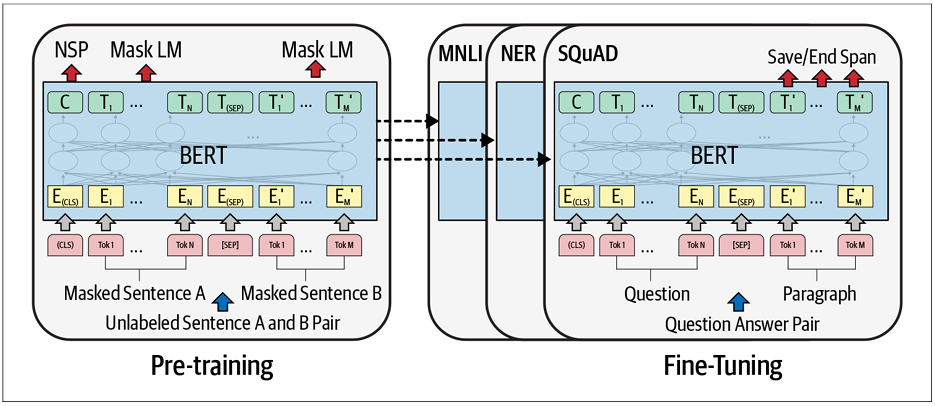
\includegraphics[angle=0,width=0.3\textwidth]{Figuras/tranformers.png}
\par \end{centering}
\caption[Transformadores]{Transformadores. \textbf{Fuente:} \cite{sowmya_practical_npl}}
\label{NLP}
\end{figure}

\subsection{Chatbots}
Los chatbots son programas que imitan la conversación humana utilizando la Inteligencia Artificial.\cite{UniversityRelatedFAQS}
\subsubsection{Características de un Chatbot}
Todos los chatbots deben contar con las siguientes cualidades. \cite{evaluating_quality}
\begin{itemize}
    \item Rendimiento: se refiere a la eficiencia en la asignación de funciones y a la robustez que tienen en cuanto a la manipulación y a las entradas inesperadas.
    \item Funcionalidad: es capaz de interpretar, responder y ejecutar  correctamente las tareas demandadas.
    \item Humanidad: la conversación con el chatbot debe ser natural, lo más parecida a la humana.
    \item Ética: genera confianza, respeta y protege la dignidad, y la privacidad de los usuarios.
    \item Accesibilidad: se encuentra disponible cuando el usuario quiera usarlo, además se refiere a que es capaz de detectar intenciones y significados
\end{itemize}
\subsubsection{Plataformas de desarrollo}
\subsection{Plataformas de desarrollo}
\begin{itemize}
    \item \textbf{DialogFlow:}
        Es la plataforma de desarrollo de chatbots de Google, permite una fácil integración a aplicaciones móviles y web, también facilita bastante el diseño de la interfaz de usuario.\\
        Admite como entrada texto y voz, es capaz de responder a los clientes con texto o voz sintética.\\\cite{Dialogflow}
    \item \textbf{IBM Watson:}
        IBM Watson  permite a los usuarios integrar sus chatbots en cualquier canal, sea web, aplicaciones o incluso una llamada.\\
        Es capaz de aprender los vocabularios de la industria,  términos coloquiales o dialectos regionales, admite entradas de voz y también de texto. \\\cite{IBMCloud2020}
    \item \textbf{Amazon Lex:}
        Amazon Lex es la propuesta del gigante tecnológico Amazon.Reconoce tanto entradas de texto como de voz, gestiona el contexto de las conversaciones de forma nativa y también permite una gran fidelidad en las interacciones de habla telefónica.\\
        Amazon Lex permite la integración con aplicaciones web, móviles y los servicios propios de Amazon como Amazon Kendra, Amazon Polly o AWS Lambda.\\\cite{Amazon_Lex}
    \item \textbf{RASA Open Source:}
    Es una plataforma de código abierto que proporciona procesamiento de lenguaje natural para convertir los mensajes de los usuarios en intenciones y entidades que los chatbots entienden, permite la gestión de los diálogos basándose en los mensajes de los usuarios y el contexto de la conversación.\\
    La integración a las aplicaciones más comunes de mensajes y a los canales de voz se puede hacer de forma muy sencilla con los conectores ya incorporados, para conectar a las demás aplicaciones móviles o web se deben personalizar los conectores.\\\cite{Rasa}
    \item \textbf{Chatterbot:}
    Chatterbot es una librería de Python que facilita la automatización de respuestas mediante  distintos algoritmos de aprendizaje automático, esto permite que una instancia de agente mejore su propio conocimiento de las posibles respuestas a medida que interactúa con humanos y otras fuentes de datos informativos\\
    Se puede integrar a las aplicaciones mediante APIs, además ChatterBot tiene soporte directo para la integración con el ORM de Django, esto facilita bastante para crear las páginas conversacionales.\cite{Chatterbot}\\
\end{itemize}

\indent Haciendo una comparación entre todas las herramientas analizadas, vemos que la creación de los chatbots con Dialogflow, IBM Watson y Amazon Lex es mucho más sencilla, ya que tienen una madurez tecnológica muy alta, gran soporte y las interfaces son muy intuitivas, además no requieren de mucha programación. La mayor desventaja es que las versiones que cuentan con todas las funcionalidades son de paga, y las versiones gratuitas son muy limitadas y básicas, por lo que descartamos estas tres opciones.\\
\indent En cuanto a Chatterbot y RASA, la curva de aprendizaje puede ser un poco mayor porque no utilizan interfaces gráficas, todo es programado con Python, un lenguaje muy versátil que cuenta con numerosas librerías, esto permite tener mayor control sobre los chatbots porque se pueden manipular todos los ficheros y modificar las configuraciones, Si bien ambos están muy bien documentados, RASA destaca de Chatterbot por su comunidad, cuenta incluso con un foro donde participan los desarrolladores y usuarios dispuestos a brindar ayuda a todo aquel que las necesite.\\
\indent Teniendo en cuenta que no contamos con experiencia en el desarrollo de chatbots, se valora de sobremanera la comunidad, documentación y tutoriales con los que cuenta RASA, además que permite la integración con distintas plataformas y el lenguaje de programación que utiliza (Python) es de nuestro conocimiento, es por eso que concluimos con que RASA es una buena elección para llevar a cabo este proyecto.
\subsection{Rasa Open Source}
Antes de profundizar en la plataforma elegida para la elaboración del proyecto, proporcionaremos algunos conceptos básicos sobre los chatbots.
\begin{itemize}
    \item \textbf{intents (intenciones): }son las categorías, denominadas utterances creadas para lo que el usuario está tratando de transmitir o lograr en una conversación. Las intenciones pueden ser divididas en pequeñas subintenciones denominadas 'Retrieval Intent'.
    \item \textbf{entities (entidades): } las entidades son informaciones o palabras clave que pueden ser extraídas de un mensaje para personalizar la conversación.
\begin{figure}[H]
\begin{centering}
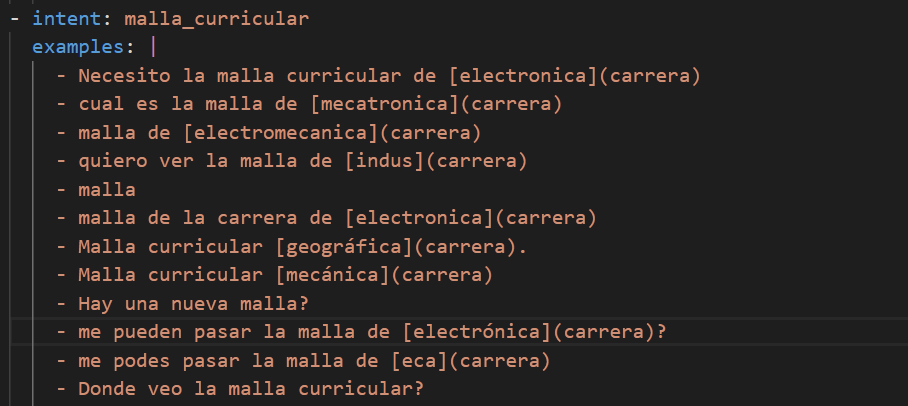
\includegraphics[angle=0,width=0.3\textwidth]{Figuras/Intent-Entities.png}
\par \end{centering}
\caption[Intenciones y Entidades]{Intenciones y Entidades. \textbf{Fuente:} Propia}
\label{Intent_Entities}
\end{figure}
    \item \textbf{slots:} es un registro de datos que Rasa utiliza para guardar la información proveída por el usuario en el curso de la conversación, un claro ejemplo del uso de este elemento es almacenar el nombre del usuario para personalizar los mensajes.
\begin{figure}[H]
\begin{centering}
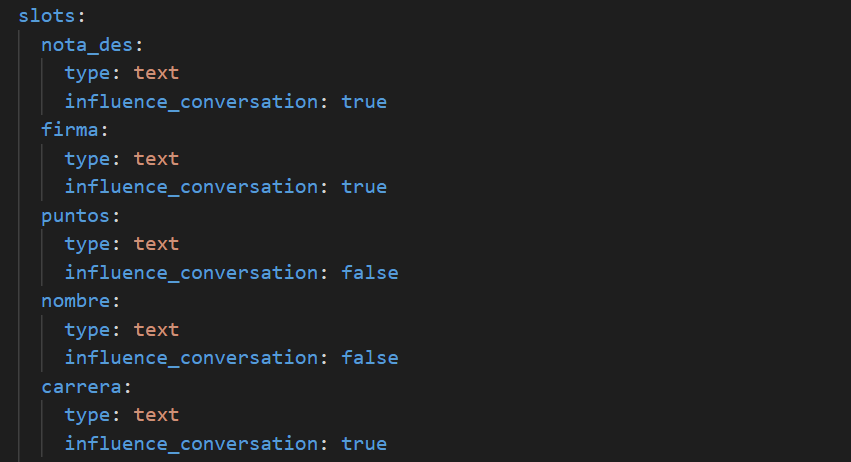
\includegraphics[angle=0,width=0.3\textwidth]{Figuras/Slots.png}
\par \end{centering}
\caption[Slots]{Slots. \textbf{Fuente:} Propia}
\label{Slots}
\end{figure}
    \item \textbf{responses (respuestas):} mensajes que los chatbots envían a los usuarios, estos pueden ser dinámicos y con cualquier tipo de contenido como texto, imágenes, links, etc.
\begin{figure}[H]
\begin{centering}
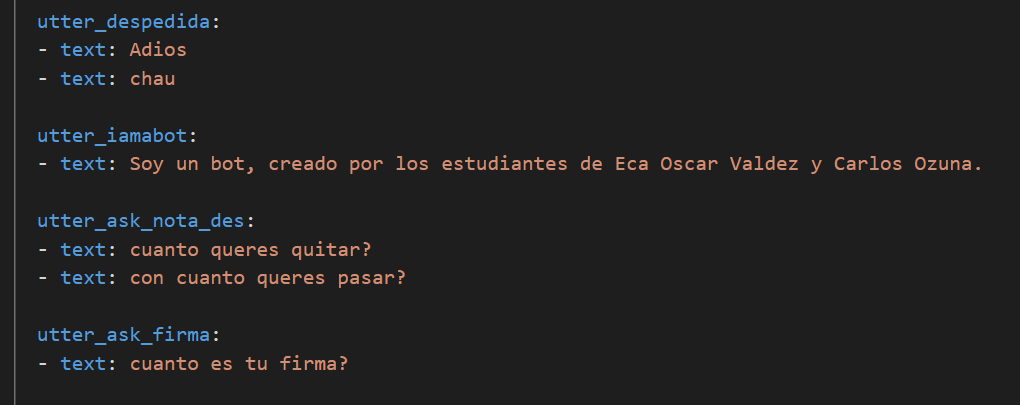
\includegraphics[angle=0,width=0.3\textwidth]{Figuras/Responses.png}
\par \end{centering}
\caption[Respuestas]{Respuestas. \textbf{Fuente:} Propia}
\label{Responses}
\end{figure}
    \item \textbf{forms (formularios):} Un tipo de acción personalizada que pide al usuario varios datos.
\begin{figure}[H]
\begin{centering}
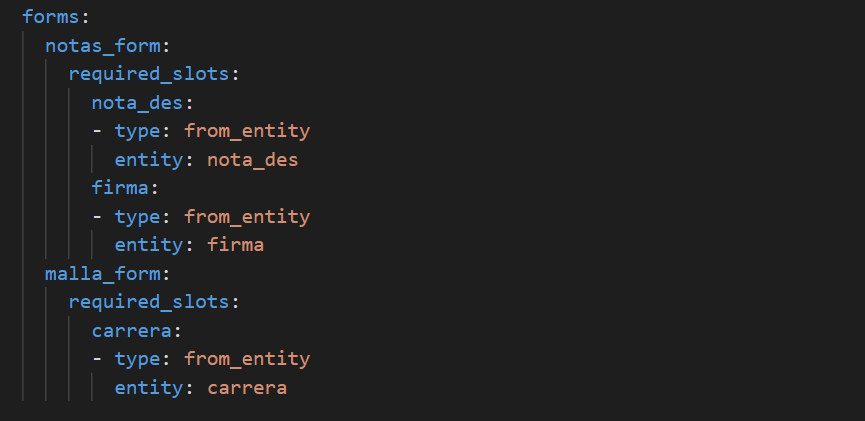
\includegraphics[angle=0,width=0.3\textwidth]{Figuras/Forms.png}
\par \end{centering}
\caption[Acciones]{Acciones. \textbf{Fuente:} Propia}
\label{Acciones}
\end{figure}
    \item \textbf{actions (acciones):} es un paso que toma el bot en la conversación por ejemplo, llamar a una API o enviar una respuesta al usuario.\cite{Glossary}
\begin{figure}[H]
\begin{centering}
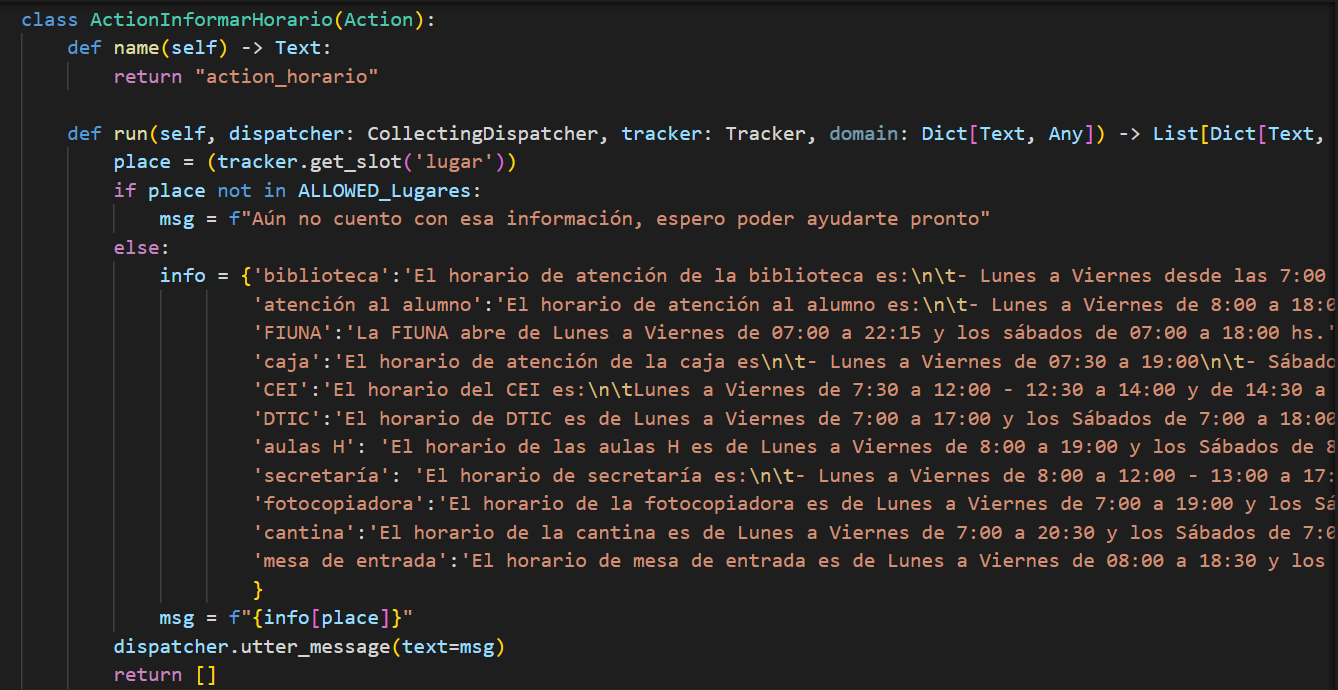
\includegraphics[angle=0,width=0.3\textwidth]{Figuras/actions.png}
\par \end{centering}
\caption[Acciones]{Acciones. \textbf{Fuente:} Propia}
\label{Actions}
\end{figure}
\end{itemize}
\subsection{¿Cómo se llevan a cabo las conversaciones?}
Para llevar a cabo las conversaciones se utilizan las dos librerías del Rasa Stack.
\begin{itemize}
    \item \textbf{Rasa NLU: } En ella  se escriben los archivos de configuración, se elige el pipeline y el modelo de entrenamiento para que deduzca las intenciones y posteriormente pueda extraer las entidades disponibles.\\
    \indent Puede ser basado en reglas o en redes neuronales, el primero suele ser más ligero y no necesita de muchos datos aunque no son buenos en tareas antes no vistas, mientras que el segundo necesita de más capacidad de cómputo y datos para entrenamiento, son más flexibles que los basados en reglas, ya que pueden aprender cosas que no han visto antes.
    \item \textbf{Rasa Core: } es el gestor de diálogos utilizado para crear modelos que sean capaces de decidir que respuestas o acciones se ejecutarán de acuerdo a las entradas generadas por el usuario.\\
    También puede ser basado en reglas, que es el enfoque más tradicional, funciona muy bien en muchos casos pero es difícil de expandir las conversaciones, también puede ser basado en redes neuronales que escoge la siguiente acción basándose en la conversación y en los ejemplos del entrenamiento.
\end{itemize}
\indent Básicamente, Rasa NLU se encarga de interpretar los mensajes y Rasa Core de de decidir que acción tomar.\\
\indent Para asegurarnos de que una conversación funcione se utiliza un proceso denominado ‘conversation-driven development’ que consiste en revisar manualmente las conversaciones para detectar cualquier error cometido, agregar nuevos datos de entrenamiento, volver a entrenar el modelo y probarlo nuevamente. \cite{Introduction_to_Rasa}
\begin{figure}[H]
\begin{centering}
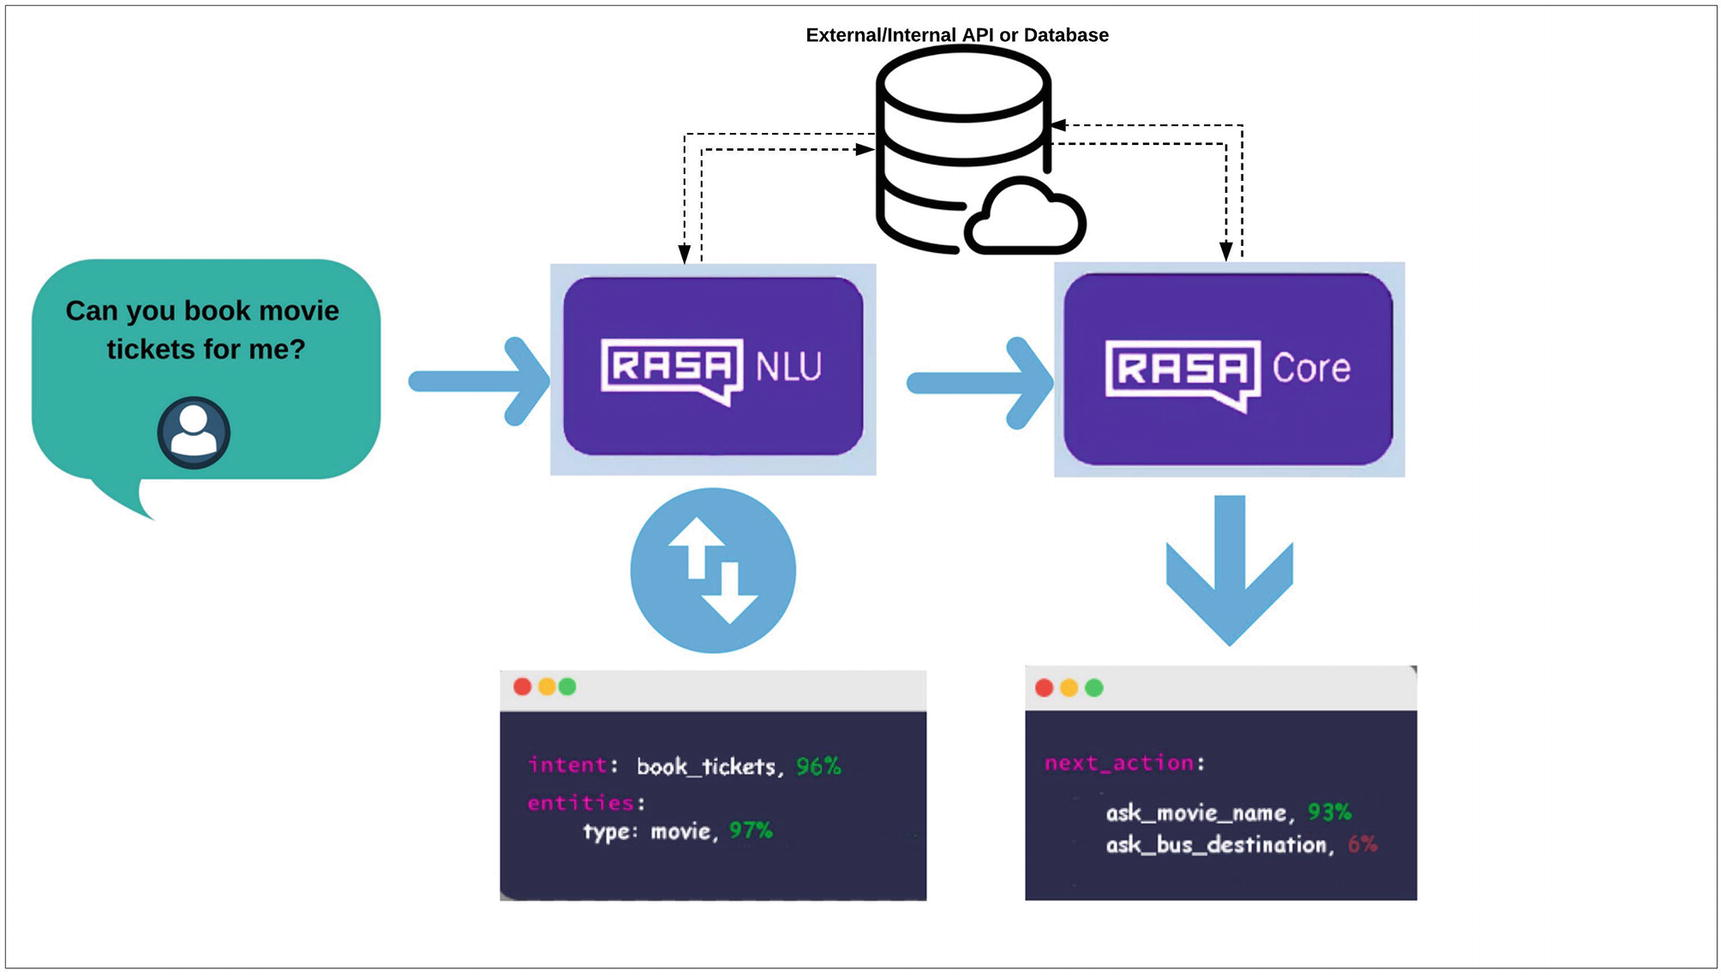
\includegraphics[angle=0,width=0.3\textwidth]{Figuras/NLU-CORE.png}
\par \end{centering}
\caption[Rasa Core y Rasa NLU]{Rasa Core y Rasa NLU. \textbf{Fuente:} \cite{Rasa_Core-NLU}}
\label{Core-NLU}
\end{figure}

\subsection{Creación del Proyecto}
La creación de un nuevo proyecto se realiza con el comando ’rasa init’, éste crea
un conjunto de carpetas y archivos así como se muestra en la siguiente figura.
\begin{figure}[H]
\begin{centering}
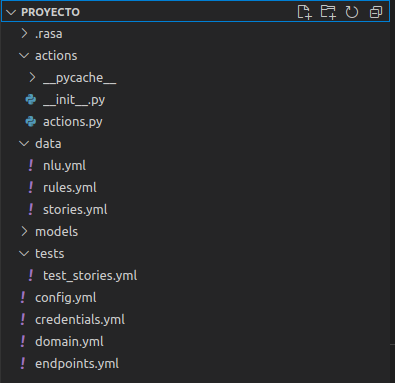
\includegraphics[angle=0,width=0.3\textwidth]{Figuras/4_Estructura del Proyecto.png}
\par \end{centering}
\caption[Estructura del Proyecto]{Estructura del Proyecto. \textbf{Fuente:} Propia}
\label{Estructura}
\end{figure}
\subsubsection{Archivo nlu}
En él se encuentran datos estructurados que sirven para entrenar el modelo y luego extraer la información de los mensajes del usuario. Estos datos son  las intenciones y entidades, también se pueden agregar expresiones regulares y algunas tablas de búsqueda. \cite{NLU_Documentation}
\subsubsection{Archivo Rules}
En este archivo se definen las reglas, que no son más que  tipo de datos de entrenamiento encargados de describir partes de una conversación que siempre sigue el mismo camino.\cite{Rules_Documentation}
\subsubsection{Archivo Stories}
Las historias son un tipo de datos de entrenamiento, se utiliza para entrenar modelos que puedan generalizar las rutas de conversación. Las entradas del usuario son expresadas mediante intents, y entitites si es necesario,  mientras que las respuestas del asistente son expresadas mediante actions.\\
Los patrones que siguen las conversaciones podemos extraer de datos ya existentes o con la herramienta de rasa 'interactive learning'. \cite{Stories_Documentation}
\subsubsection{Archivo config}
En el archivo config se definen el lenguaje y los componentes del pipeline, que forman parte de Rasa NLU y las políticas a ser utilizadas, correspondiente a Rasa NLU.\\
El pipeline es el encargado de definir la dirección de flujo de datos entre los diferentes componentes, Rasa nos permite configurar cada uno de ellos según nuestras necesidades, de tal forma que podamos realizar las predicciones de las intenciones y la extracción de las entidades. Las políticas forman parte de la gestión de diálogos, encargada de seleccionar la siguiente acción a ser ejecutada. \cite{Configuration_Documentation}
La configuración del pipeline y las políticas son de suma importancia, por lo que se detallaran sus componentes en otra sección.
\subsubsection{Archivo credentials}
Aquí se definen los credenciales para las plataformas de voz y chat que el bot utiliza. Rasa cuenta con algunos conectores preestablecidos para los canales más conocidos como Facebook Messenger, Telegram, Google Hangouts Chat o una pagina web propia. \cite{Credentials_Documentation}
\subsubsection{Archivo domain}
El archivo domain es un archivo de configuración donde se especifican las intenciones, entidades, slots, respuestas, formularios y acciones que el bot debe saber. \cite{Domain_Documentation}
\subsubsection{Archivo endpoints}
Los endpoints son los enlaces a los servicios externos o internos que puede tener Rasa. En el se definen los servidores que corren o en los que están alojadas las acciones personalizadas, al igual que los modelos con los que se cuenta. También es aquí donde se especifican los tracker store, utilizados para guardar las conversaciones, y los event broker, encargados de conectar el bot con otros servicios que procesan los datos que llegan de las conversaciones.
\subsection{Componentes}
En esta sección estaremos describiendo el funcionamiento de los componentes
utilizados en la arquitectura de Rasa, estos componentes son modulares y genéricos para lo que son sistemas de NLU modernos, pueden ser propios del entorno
o proveídos por otras librerías de terceros para extender funcionalidades
\begin{figure}[H]
\begin{centering}

\includegraphics[angle=0,width=0.3\textwidth]{Figuras/Componentes_NLU.png}
\par \end{centering}
\caption[Componentes del NLU]{Componentes del NLU. \textbf{Fuente:} Propia}
\label{Estructura}
\end{figure}
\subsubsection{Tokenizadores}
Antes de poder ser procesada una porción de texto debe ser dividida en porciones más pequeñas, para esto se utiliza 
un tokenizador (o tokenizer).   Este divide el texto en componentes de un vector.
\subsubsection{Caracterizadores}
Los caracterizadores generan pesos numéricos para ser consumidos por los modelos de ML. Existen dos tipos principales de
características, las Dispersas (Sparse Features) que pueden representar subpalabras o características
léxicas, estas son las utilizadas para que aprendan los significados del dominio, y las Densas (Dense Features) que suelen consistir en porciones preentrenadas, útiles especialmente al iniciar un proyecto y no se cuenta con suficientes datos de entrenamiento.
\begin{table}[h]
\resizebox{0.49\textwidth}{!}{%
\begin{tabular}{|l|l|l|}
\hline
\textbf{Caracterizador}    & \textbf{Requisitos}     & \textbf{Tipo}                                                                  \\ \hline
MitieFeaturizer            & MitieNLP                & Dense featurizer                                                               \\ \hline
SpacyFeaturizer            & Dense / Sparse Features & \begin{tabular}[c]{@{}l@{}}Logistic Regression de \\ scikit-learn\end{tabular} \\ \hline
ConveRTFeaturizer          & Tokenization            & Dense featurizer                                                               \\ \hline
LanguageModelFeaturizer    & Tokenization            & Dense featurizer                                                               \\ \hline
CountVectorsFeaturizer     & Tokenization            & Sparse featurizer                                                              \\ \hline
LexicalSyntactitFeaturizer & Tokenization            & Sparse featurizer                                                              \\ \hline
RegexFeaturizer            & Tokenization            & Sparse featurizer                                                              \\ \hline
\end{tabular}%
}
    \caption{ Caracterizadores. Elaboración Propia}
    \label{tab:Caracterizadores}
\end{table}
\subsubsection{Extractor de Entidades}
Los extractores de entidades son herramientas que se utilizan para identificar y extraer información relevante de un texto, como son los nombres, lugares o números. Dependiendo de la situación, puede ser implementado un extractor basado en Expresiones
Regulares o extractores basados en Aprendizaje Automático.
\begin{table}[h]
\resizebox{0.49\textwidth}{!}{%
\begin{tabular}{|l|l|l|}
\hline
\textbf{Clasificador}   & \textbf{Requisitos} & \textbf{Utiliza}                                                            \\ \hline
MitieEntityExtractor    & MitieNLP            & \begin{tabular}[c]{@{}l@{}}Clasificación multi-clase \\ con SVM\end{tabular} \\ \hline
SpacyEntityExtractor    & SpacyNLP            & Modelo estadístico BILOU                                                    \\ \hline
CRFEntityExtractor      & Tokens              & Campo aleatorio condicional (CRF)                                           \\ \hline
DucklingEntityExtractor & Ninguno             & Expresiones regulares                                                       \\ \hline
DIETClassifier          & Dense Features      & Transformadores                                                             \\ \hline
RegexEntityExtractor    & Ninguno             & Tablas de búsqueda                                                          \\ \hline
\end{tabular}%
}
\caption{Extractores de entidades. Elaboración propia}
\label{EntityExtractor}
\end{table}
\subsubsection{Clasificador de Intenciones}
Una vez que se generaron las características para todos los tokens y para toda la oración, podemos pasarlos a un
modelo clasificador de intenciones para obtener la intención detrás de cada mensaje de usuario y posteriormente poder brindarle una respuesta adecuada.
\begin{table}[h]
\resizebox{0.49\textwidth}{!}{%
\begin{tabular}{|l|l|l|}
\hline
\textbf{Clasificador}        & \textbf{Requisitos}     & \textbf{Utiliza}                                                                              \\ \hline
MitieIntentClassifier        & MitieNLP                & Clasificación multiclase con SVM                                                              \\ \hline
LogisticRegressionClassifier & Dense / Sparse Features & Logistic Regression de scikit-learn                                                           \\ \hline
SklearnIntentClassifier      & Dense Features          & \begin{tabular}[c]{@{}l@{}}SVM lineal optimizado con búsqueda \\ en cuadrícula\end{tabular}   \\ \hline
KeywordIntentClassifier      & Ninguno                 & Comparador de palabras clave                                                                  \\ \hline
DIETClassifier               & Dense Features          & Transformadores                                                                               \\ \hline
FallbackClassifier           & Intents                 & \begin{tabular}[c]{@{}l@{}}Requiere de un clasificador de \\ intenciones previo\end{tabular} \\ \hline
\end{tabular}%
}

\caption{Clasificadores de intenciones. Elaboración propia}
\label{IntentClassifier}
\end{table}
 \subsection{Predicción de Acciones}
Con el flujo NLU, se detectan las entidades e intenciones. Pero este flujo no predice la siguiente acción en la 
conversación. Para esto se utiliza el flujo de política. Las políticas aseguran el uso de predicciones de NLU así como 
también el estado presente de la conversaciones para decidir que acción tomar, pueden ser basado en reglas o en aprendizaje automático.
\textbf{Políticas basadas en Aprendizaje Automático:}
\begin{itemize}
    \item \textbf{TED Policy:}
    Es un conjunto de algoritmos desarrollados por RASA para la predicción de diálogo y reconocimiento de entidades. Su arquitectura se basa en transformadores que convierten el diálogo actual en un vector de diálogos, para compararlos con otros vectores en busca del más cercano, a partir de las acciones existentes.\cite{TED_Policy}
    \item \textbf{UnexpecTED Intent Policy:} Es una política auxiliar, tiene la misma arquitectura que TEDPolicy pero éste aprende cuales son las intenciones más probables a ser expresadas según el contexto de la conversación. Siempre debe usarse en conjunto con al menos una otra política.\cite{UnexpecTED}
    \item \textbf{Memoization Policy: }Esta política utiliza las historias y acciones de los datos de entrenamiento y las guarda en un diccionario, si la conversación actual no coincide con ningún ejemplo, predice un 0.0, se aplica cuando la los datos ingresados son similares a un historia existente.\cite{MemoizationPolicy}
    \item \textbf{Augmented Memoization Policy: } Tiene las mismas funcionalidades de Memoization Policy, pero además cuenta con un mecanismo que permite olvidar de forma aleatoria algunas partes de la conversación, luego predice las acciones ya con la historia reducida.\cite{AugmentedMemoizationPolicy}
\end{itemize}
\textbf{Políticas basadas en Reglas:}
\begin{itemize}
    \item \textbf{Rule Policy:} Realiza las predicciones basándose en reglas que se tienen en los datos de entrenamiento.
\end{itemize}
\indent Con cada interacción, las políticas definidas indican con un nivel de confianza cuál será la siguiente acción a ser tomada, aquella que tiene obtiene el mayor resultado será la que decida la siguiente acción, en caso de que se prediga con la misma confianza, se tiene en cuenta la siguiente asignación de importancia.
\begin{itemize}
    \item 6 - RulePolicy
    \item 3 - MemoizationPolicy o AugmentedMemoizationPolicy
    \item 2 -  UnexpecTEDIntentPolicy
    \item 1 - TEDPolicy
\end{itemize}
